\documentclass[11pt]{article}

\usepackage[margin=1in]{geometry}
\usepackage{graphicx}
\usepackage{booktabs}
\usepackage{array}
\usepackage{amsmath}
\usepackage{caption}
\usepackage{float}
\usepackage[hidelinks]{hyperref}
\usepackage[round]{natbib}

\graphicspath{{../figures/}}
\setlength{\parskip}{0.45em}
\setlength{\parindent}{0pt}
\captionsetup{font=small, labelfont=bf}

\title{\textbf{Mapping Cultural Access Gaps in Chicago}\\
\large A GIS Analysis of Museums, Galleries, and Arts Centers}
\author{Felix Liu \and Qi Liu \and Zhiyuan Zhou}
\date{PPHA 38520 Final Project\\May 2026}

\begin{document}
\maketitle

\begin{abstract}
This project asks whether museums and related cultural institutions in Chicago are spatially distributed in a way that provides equitable neighborhood access. We combine 2024 American Community Survey tract data, 2024 TIGER/Line tract geometry, official Chicago community-area boundaries, CTA rail-stop context, and an OpenStreetMap inventory of museums, galleries, and arts centers. The analysis measures tract-level proximity to cultural institutions using representative-point distance, maps citywide access patterns in QGIS, compares access across demographic groups, and estimates a population-weighted tract model. The results show that cultural institutions are strongly clustered and that access gaps are clearest for majority Black and majority Hispanic tracts and for outer South, West, Northwest, and Southwest Side community areas. About 65.3 percent of Chicago's population lives within one mile of a broad cultural institution, but only 48.8 percent lives within one mile of a museum-only location. The broad conclusion is that Chicago's cultural access problem is not simply a poverty gradient or a car-ownership gradient; it is a spatial and racialized geography of institutional concentration, centrality, and edge-neighborhood exclusion.
\end{abstract}

\section{Research Question and Hypotheses}

Chicago is often described as a city rich in museums and cultural institutions, but a citywide count does not tell us whether those institutions are accessible from all neighborhoods. This project asks: \textbf{Are museums and cultural institutions in Chicago spatially distributed in a way that provides equitable neighborhood access, or do cultural-access gaps align with income, race and ethnicity, poverty, and transportation disadvantage?}

The central hypothesis is that museums and cultural institutions are concentrated in downtown, lakefront, North Side, and tourist-oriented areas, while some South Side, West Side, Northwest Side, and Southwest Side communities have weaker nearby access. We test four specific hypotheses. First, cultural institutions will be spatially clustered rather than evenly distributed. Second, high-poverty tracts and majority Black or Hispanic tracts will have longer average access times than lower-poverty or majority White tracts. Third, museum-only access will be more unequal than access to a broader universe that includes galleries and arts centers. Fourth, car-ownership disadvantage will not necessarily predict poor access by itself, because many no-vehicle households are located in dense central and transit-rich neighborhoods.

\section{Literature and Background}

Research on cultural participation increasingly treats place as part of the opportunity structure for arts access. \citet{brook2016} shows this directly for London: access to museums and galleries is associated with museum attendance even after accounting for individual social stratification. That finding motivates the present study's core assumption that museum geography matters independently of individual interest or educational background.

Foundational accessibility theory gives that assumption a broader planning basis. \citet{hansen1959} defines accessibility as the potential for interaction between places and opportunities, which makes museum geography a question about the distribution of cultural opportunity rather than only the location of individual facilities. \citet{geurs2004} also stress that accessibility has multiple components, including land use, transportation, time, and individual constraints. Their framework is useful here because it clarifies what this project can and cannot measure: tract-to-institution proximity captures the spatial-opportunity component of cultural access, but not the full lived experience of reaching, affording, entering, or feeling welcome in an institution.

Recent GIS studies also show that cultural access can be measured as a spatial equity problem. \citet{moldavanova2021} develop an index of access to cultural amenities in metropolitan Detroit using distance, transportation availability, and admission factors. Their study is especially relevant because it treats cultural amenities as neighborhood infrastructure and finds that historically underrepresented populations often face lower access to galleries, museums, and performing arts institutions. \citet{zhao2023} compare museum accessibility in Seoul and Tokyo and show that walking accessibility depends not only on where museums are located, but also on how museum locations fit the surrounding urban structure. \citet{chen2025} similarly propose a GIS framework for cultural-resource equity using spatial distribution, accessibility, and low-income-community measures.

This project is closest to \citet{moldavanova2021}, but it fills a slightly different gap. Their Detroit study builds a richer multidimensional index across a metropolitan region, while this Chicago study uses a narrower proximity measure in exchange for a sharper racial-equity and neighborhood-geography lens within one city. That tradeoff lets the analysis ask whether formal and semi-formal cultural infrastructure is clustered in ways that disadvantage majority Black and majority Hispanic tracts, and whether the answer changes when the institution universe expands beyond museums alone. In that sense, the project complements a comprehensive access-index approach with a more local cultural equity audit.

Together, this literature implies three design choices. First, a cultural equity study should not stop at mapping points; it should connect those points to residential geography. Second, access measures should be named honestly, distinguishing proximity from full realized accessibility. Third, access should be tested under more than one institution definition. A museum-only inventory captures formal cultural infrastructure, while a broader inventory recognizes galleries and arts centers that may provide more neighborhood-scale cultural opportunities.

\section{Data and Methods}

The study area is the City of Chicago. Census tracts are the primary analytical unit because recent American Community Survey (ACS) data are available at that scale. Community areas are used for interpretation because they are official and locally legible. We use 2024 ACS five-year estimates for population, median household income, poverty, race, Hispanic origin, no-vehicle households, and public-transit commuting. Tract geometries come from 2024 TIGER/Line files, and community-area boundaries come from the City of Chicago data portal. Institution points are extracted from OpenStreetMap through Overpass on May 6, 2026. The QGIS project also includes CTA rail-stop points as transit context.

The institution inventory has two definitions. The \textit{museum-only} universe includes OSM features tagged \texttt{tourism=museum}. The \textit{broad cultural-institution} universe includes those museums plus \texttt{tourism=gallery}, \texttt{amenity=arts\_centre}, and \texttt{amenity=arts\_center}. After filtering to Chicago and deduplicating repeated names at nearly identical locations, the final inventory contains 163 broad cultural institutions: 71 museums, 49 galleries, and 43 arts centers.

All distance calculations use NAD83 / UTM zone 16N (EPSG:26916). Following \citet{geurs2004}, we treat the main metric as a land-use/proximity measure of accessibility, not a complete person-based or transit-based measure. For each tract, we calculate the distance from the tract representative point to the nearest institution and convert that distance to a simple walking-time proxy at 3 miles per hour. This is defensible for a first citywide equity screen because it is transparent, consistent across all tracts, and directly tied to the geography of cultural opportunities. It is also limited: it is not a street-network travel time, does not use GTFS schedules, and does not capture hours, admission cost, disability access, or perceived safety. We also count institutions within 0.5, 1, and 2 miles of each tract representative point and mark whether a tract has at least one institution within one mile.

The analysis has four parts. First, we map the distribution of institutions and calculate a nearest-neighbor clustering statistic. Second, we map tract-level broad access and a bivariate poverty/access classification in QGIS. Third, we compare population-weighted access across demographic groups. Fourth, we estimate a population-weighted ordinary least squares model with robust standard errors:
\[
\begin{aligned}
\text{BroadWalkMin}_i ={}& \alpha + \beta_1\text{Poverty}_i
 + \beta_2\text{NoVehicle}_i + \beta_3\text{BlackShare}_i \\
&+ \beta_4\text{HispanicShare}_i
 + \beta_5\log(\text{Income}_i) + \beta_6\text{Density}_i
 + \beta_7\text{LoopDistance}_i + \epsilon_i .
\end{aligned}
\]
The model is descriptive rather than causal; its purpose is to test whether demographic associations remain after accounting for urban density and distance from the Loop.

\section{Findings}

Figure~\ref{fig:distribution} shows the first major finding: Chicago's museums, galleries, and arts centers are clustered, especially in and around the Loop, Near North Side, Near West Side, Lincoln Park, Hyde Park, and selected lakefront corridors. The broad-institution nearest-neighbor ratio is 0.70 using a convex-hull reference area, indicating a clustered rather than random point pattern.

\begin{figure}[H]
    \centering
    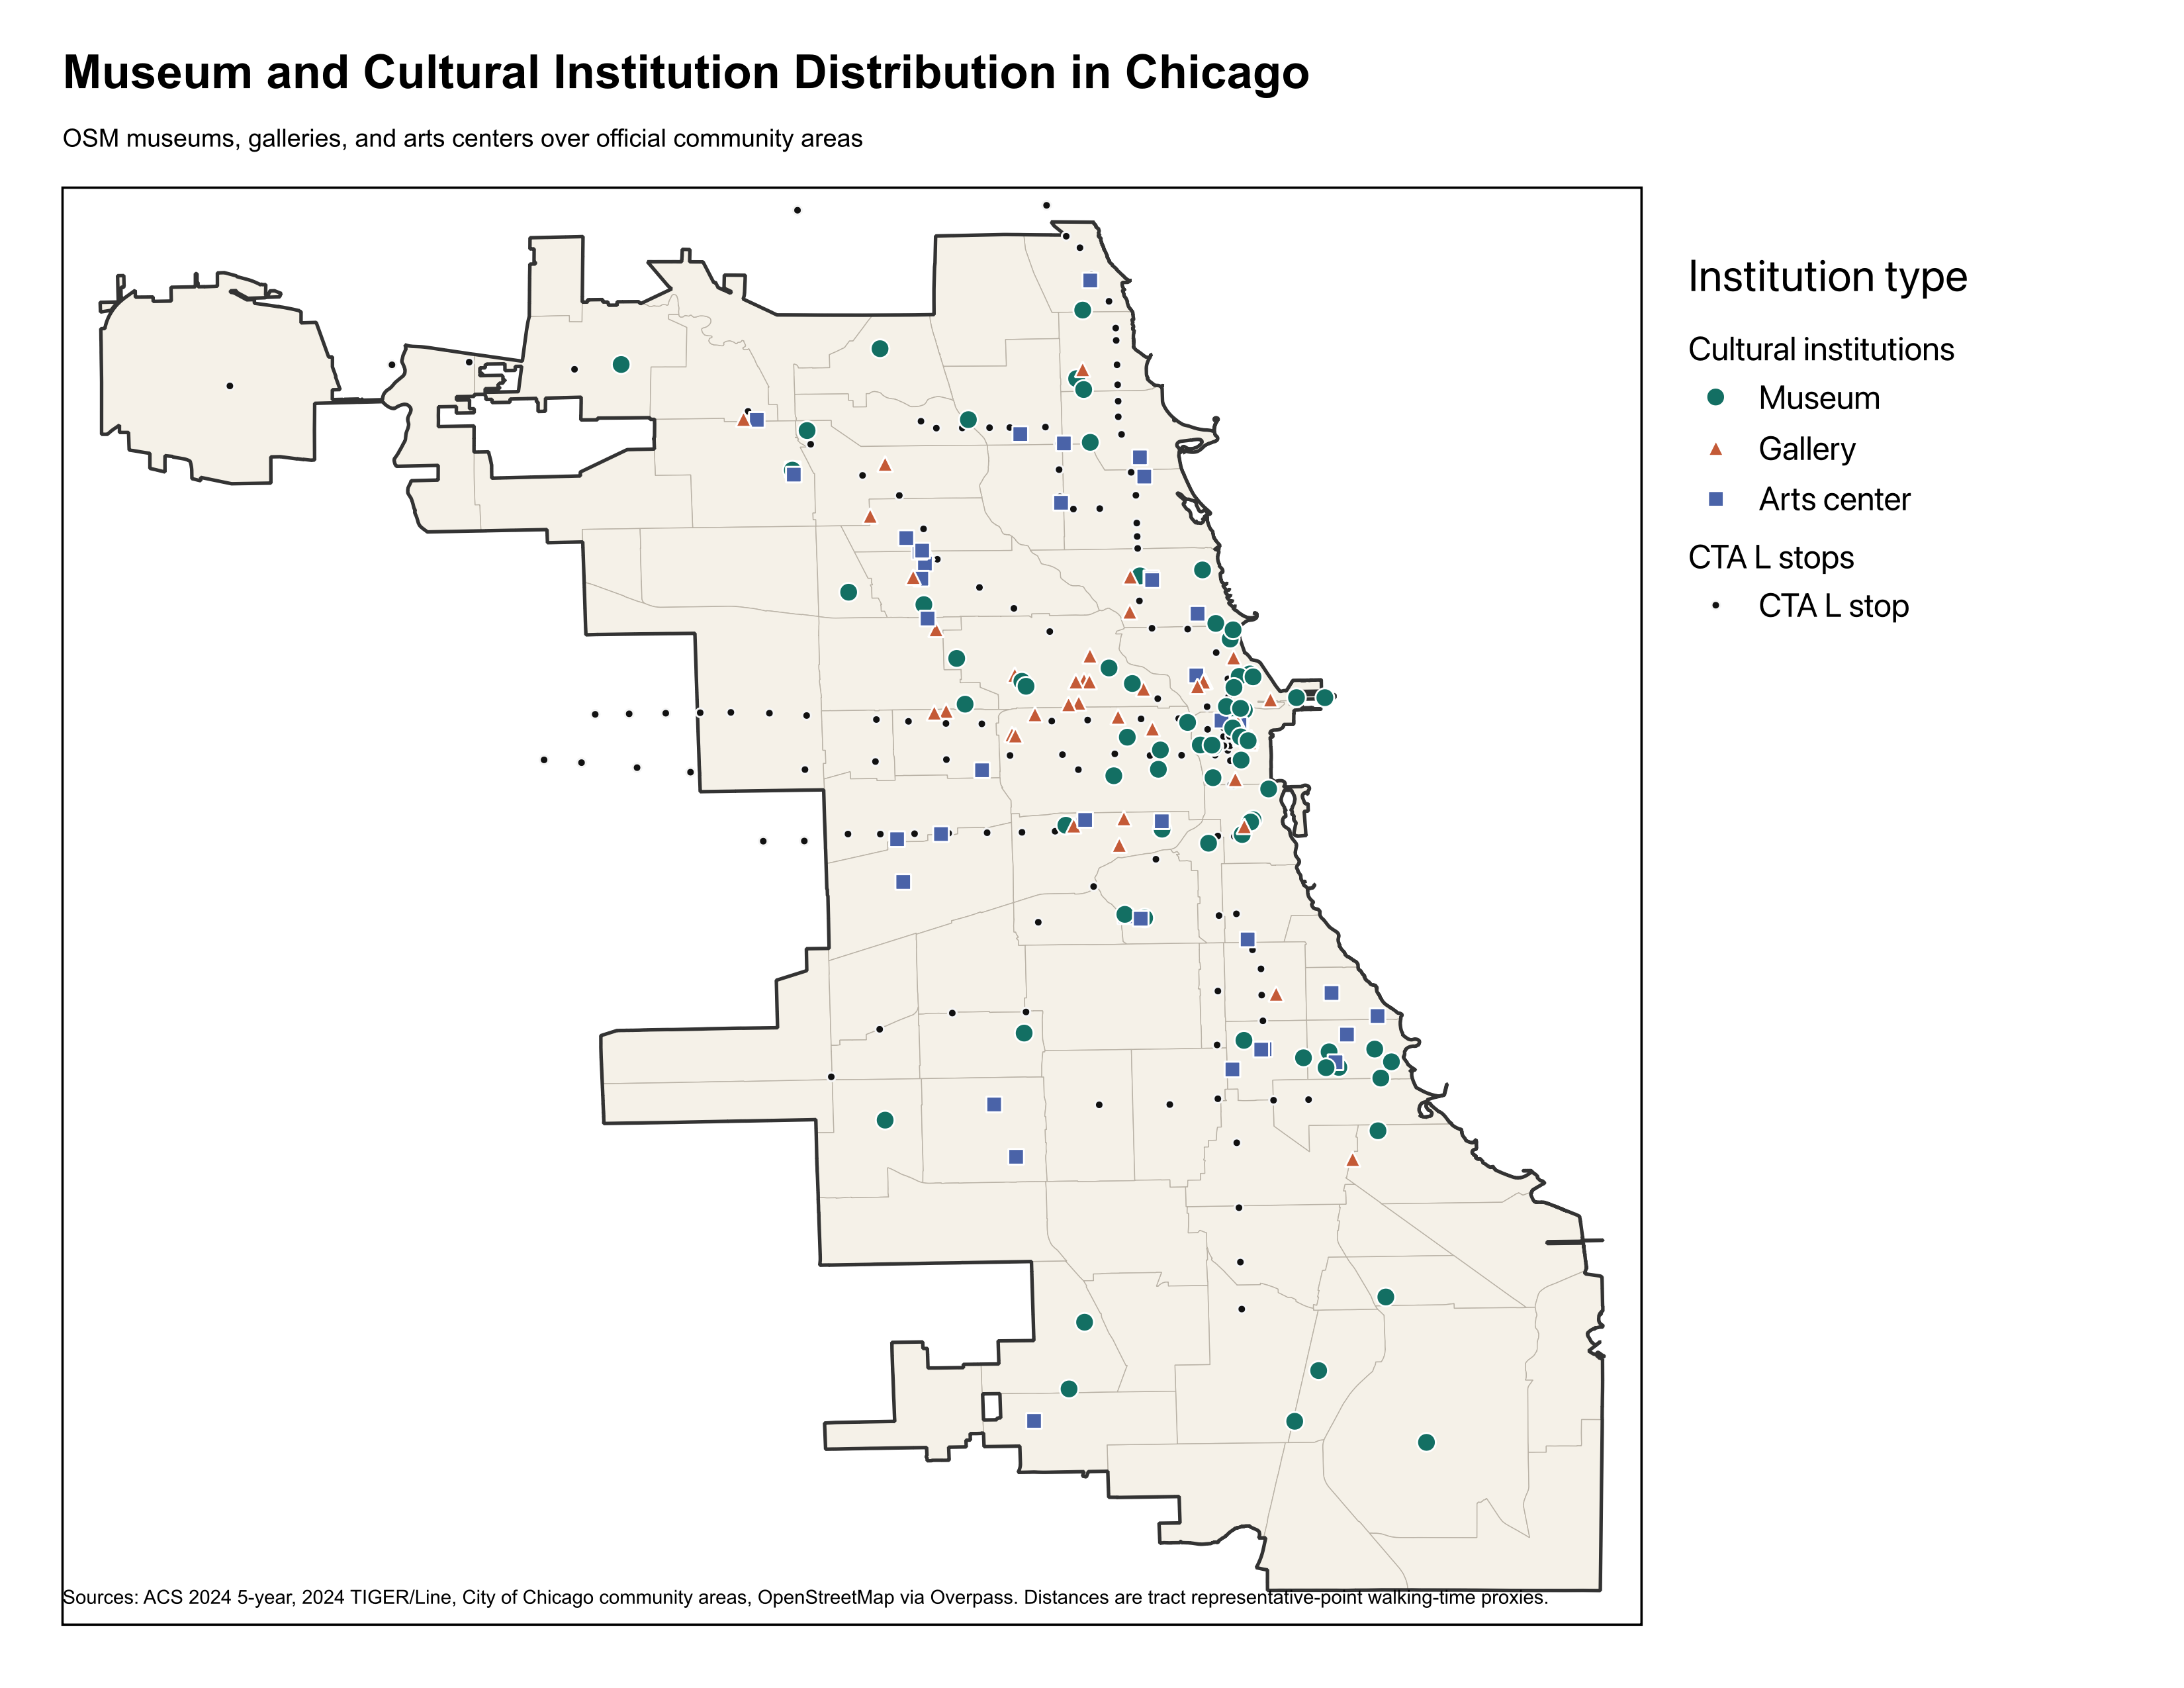
\includegraphics[width=\textwidth]{fig_01_institution_distribution_qgis.png}
    \caption{Museum, gallery, and arts-center locations in Chicago. Map produced in QGIS from OpenStreetMap, City of Chicago, and CTA layers.}
    \label{fig:distribution}
\end{figure}

The tract access map in Figure~\ref{fig:broadaccess} shows that access is strongest near the central city and several lakefront or university-linked areas. Long walking-time proxies appear in far Northwest and Southwest Side tracts, portions of the West Side, and several far South and Southeast Side communities. The pattern is not simply a North-South divide: some South Side areas near Hyde Park, Washington Park, Grand Boulevard, and Bronzeville have short access times, while some lower-poverty outer communities such as Montclare, Dunning, Garfield Ridge, and Clearing have long distances.

\begin{figure}[H]
    \centering
    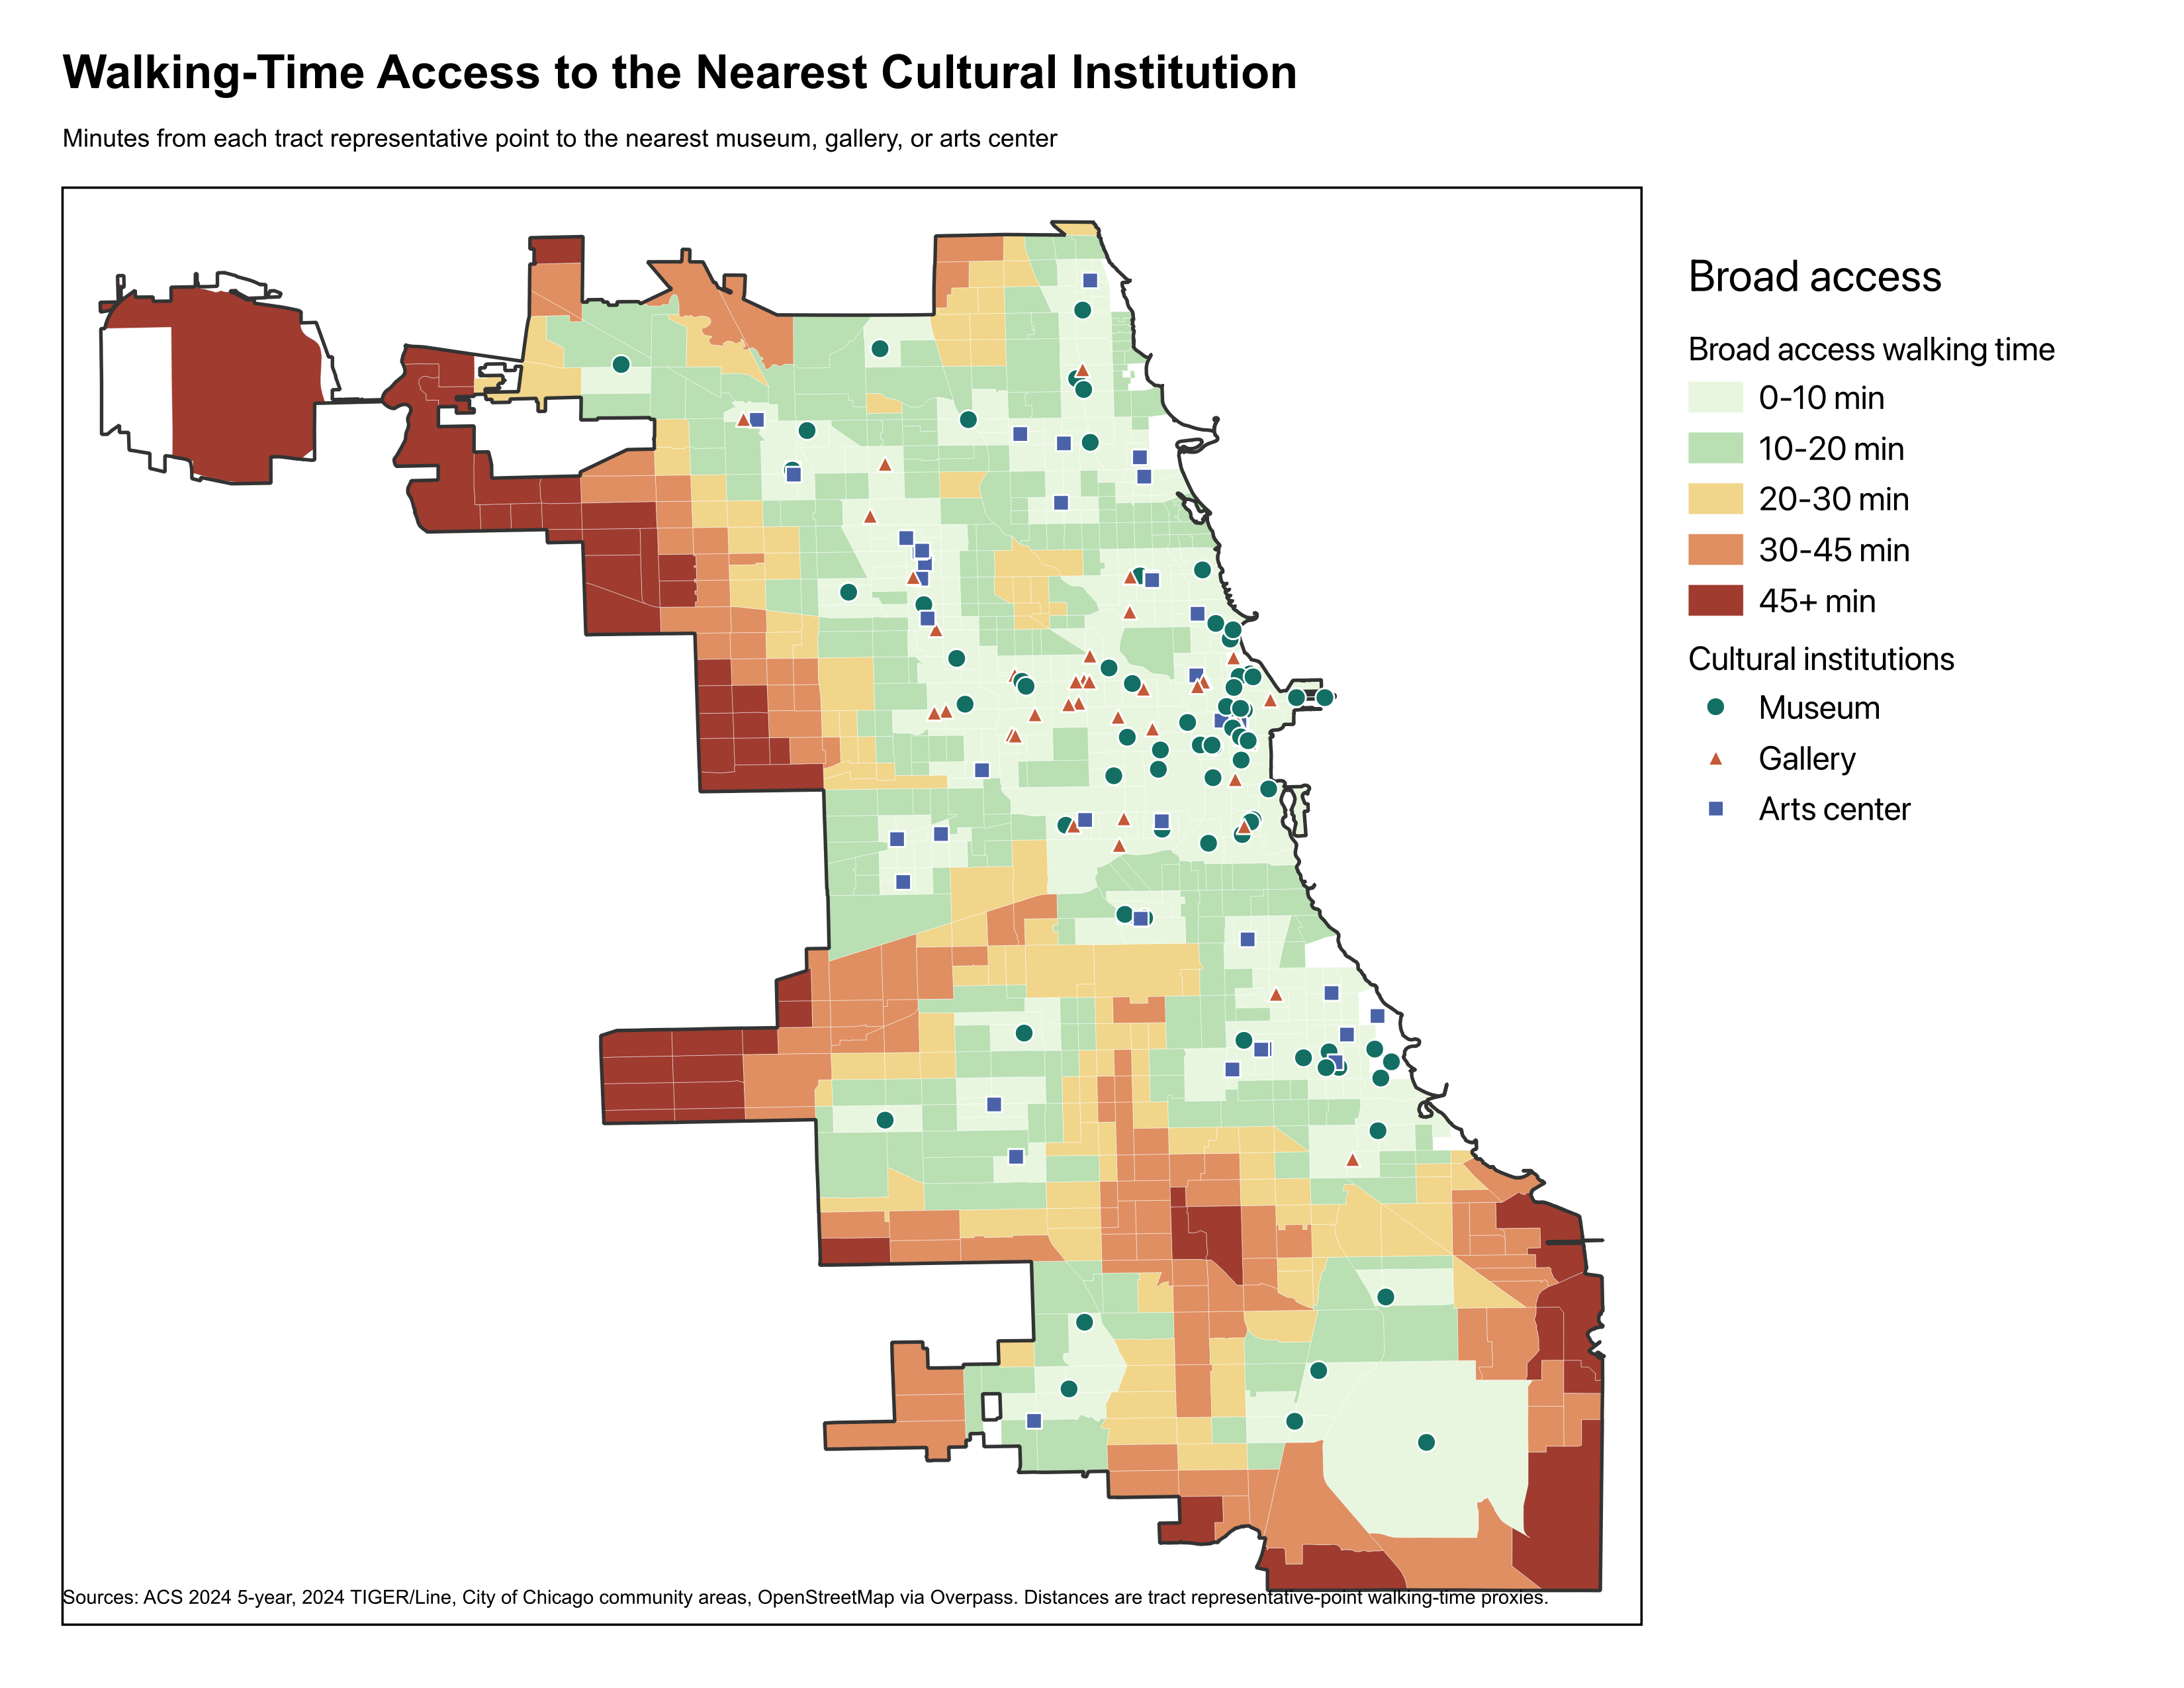
\includegraphics[width=\textwidth]{fig_02_broad_access_tracts_qgis.png}
    \caption{Tract-level walking-time proxy to the nearest broad cultural institution.}
    \label{fig:broadaccess}
\end{figure}

The bivariate map in Figure~\ref{fig:bivar} highlights where high poverty and long access coincide. The most concerning combined gaps appear in parts of the West Side and South Side, including areas around Austin, South Chicago, Riverdale, and nearby communities. However, the map also shows why the results cannot be reduced to poverty alone: some high-poverty tracts near central cultural clusters have short access, while some lower-poverty outer neighborhoods have long access.

\begin{figure}[H]
    \centering
    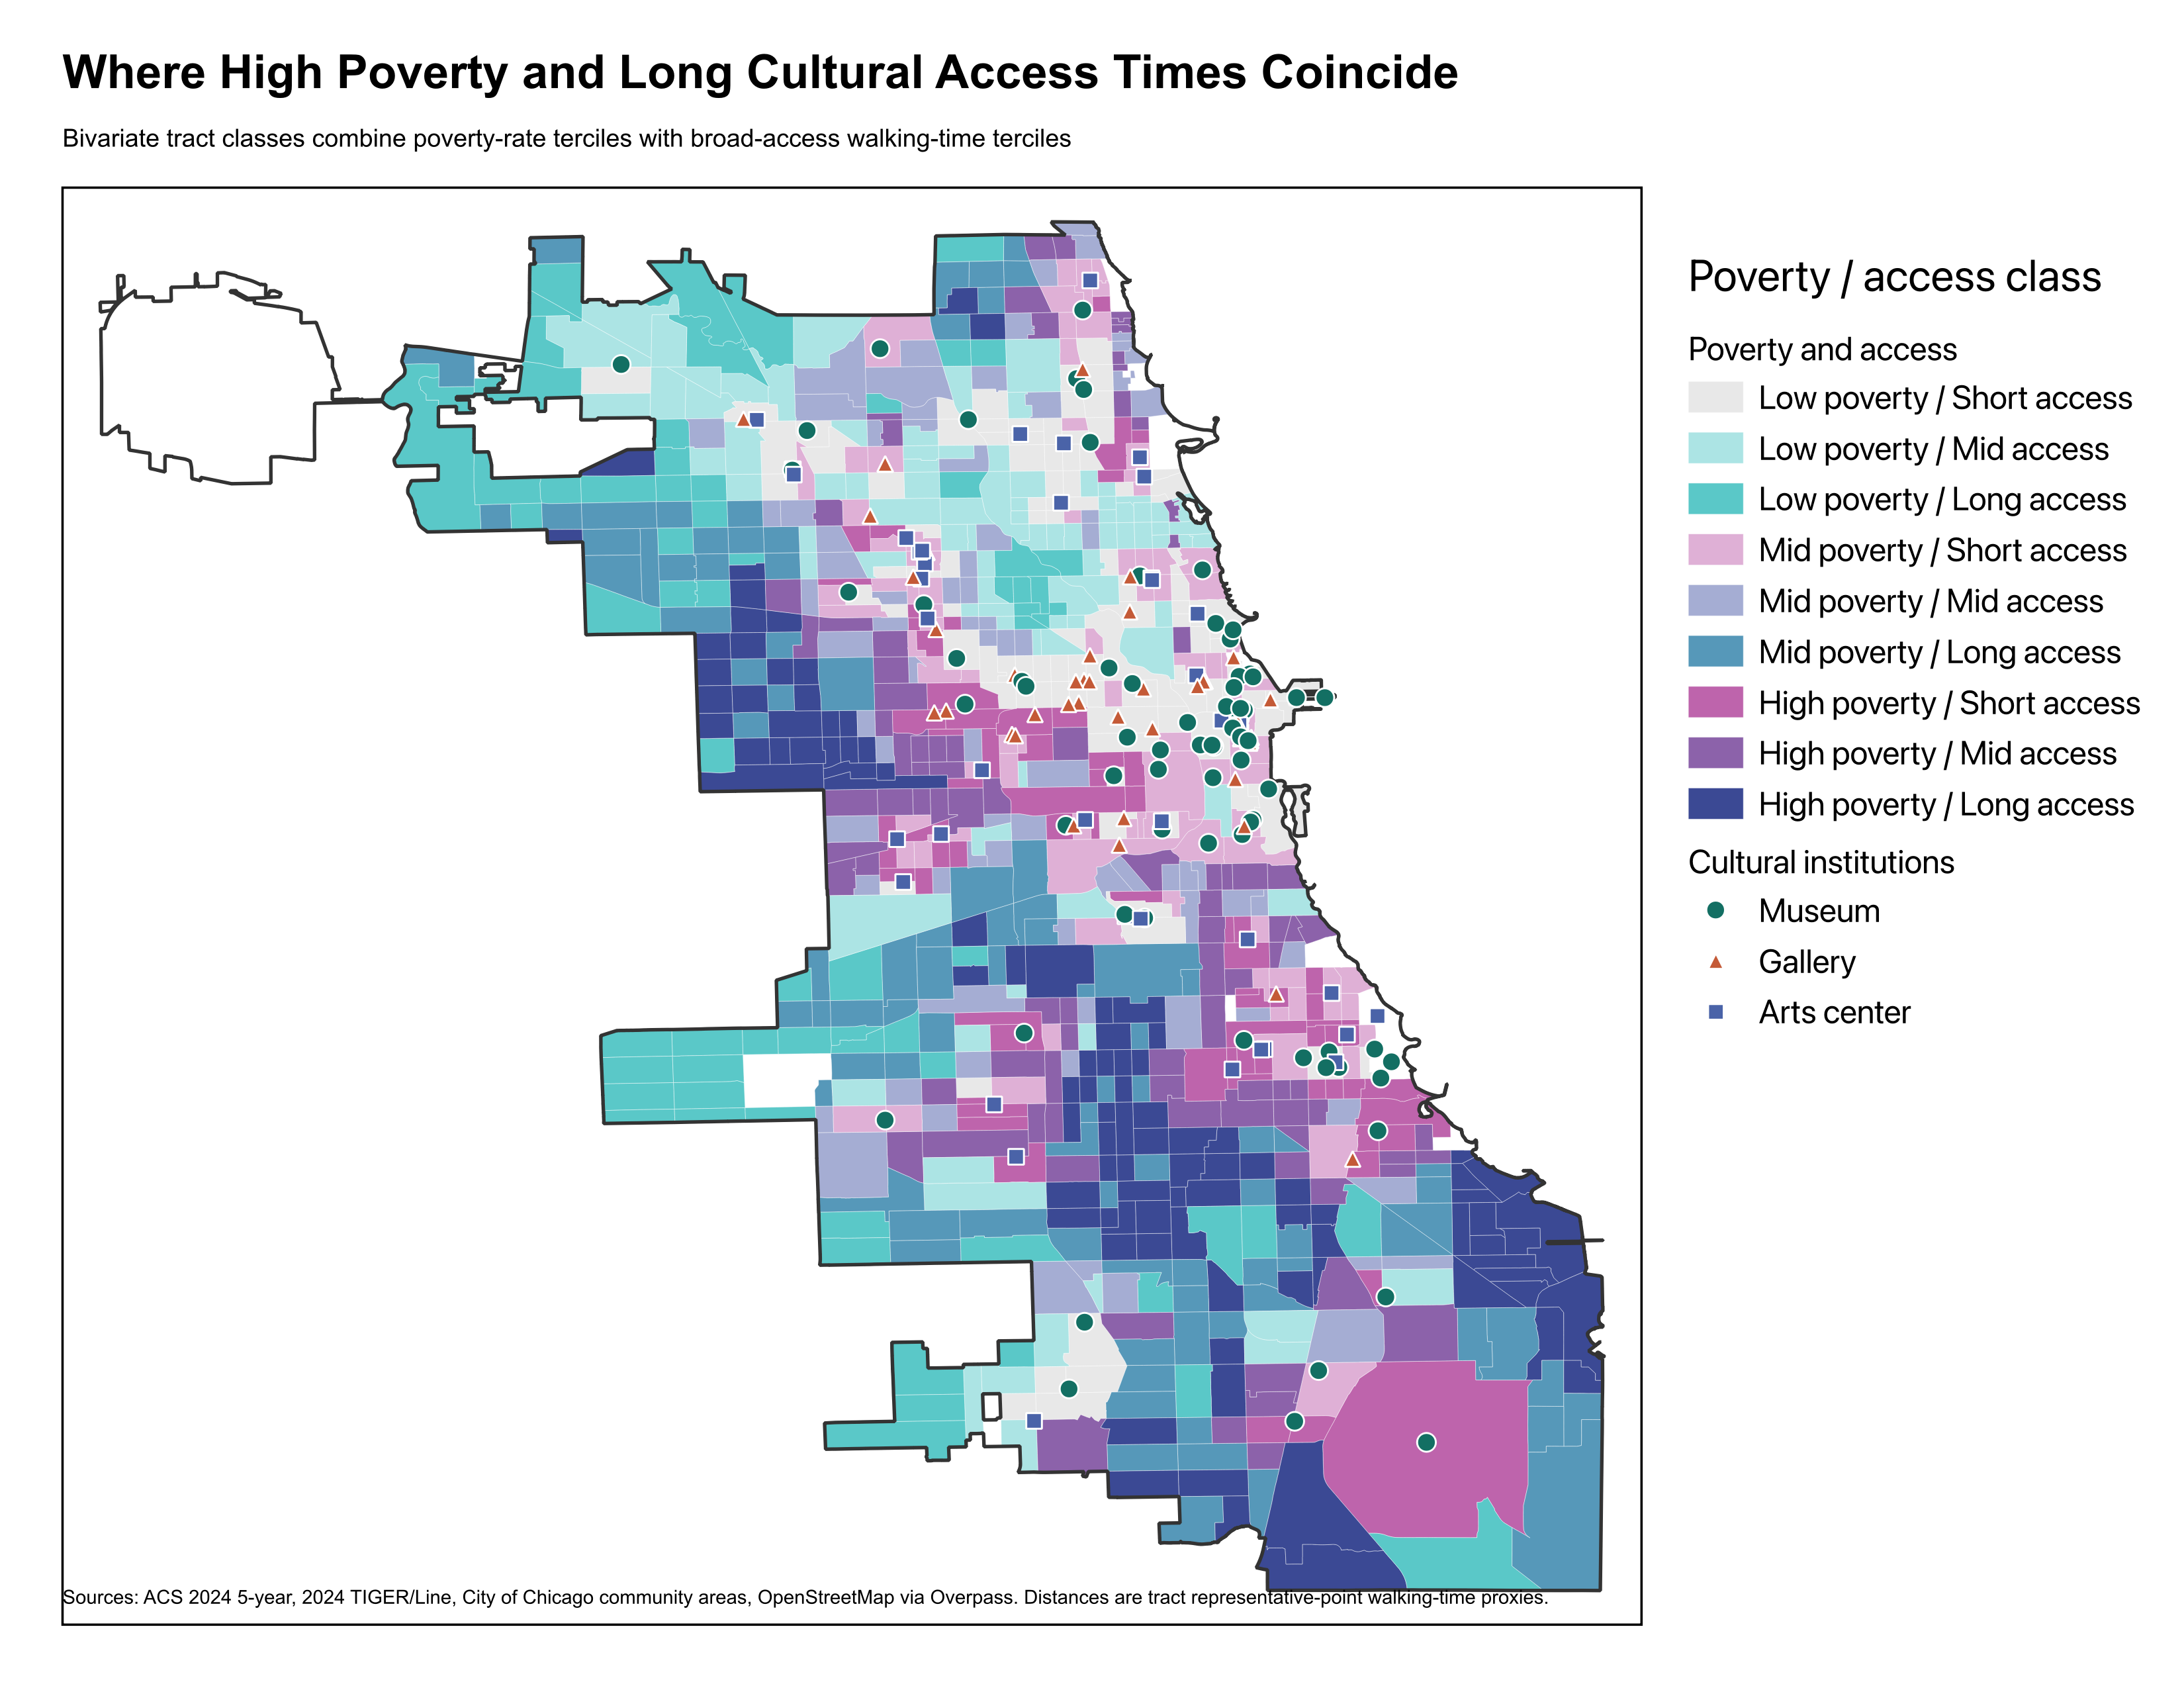
\includegraphics[width=\textwidth]{fig_03_poverty_access_bivariate_qgis.png}
    \caption{Bivariate map of poverty terciles and broad cultural-access walking-time terciles.}
    \label{fig:bivar}
\end{figure}

Table~\ref{tab:groups} summarizes the population-weighted access differences. Citywide, the average resident is about 18.8 walking minutes from the nearest broad cultural institution and 23.8 minutes from the nearest museum-only institution. About 65.3 percent of residents are within one mile of a broad institution, compared with 48.8 percent within one mile of a museum-only site.

\begin{table}[H]
\centering
\caption{Population-weighted cultural access by tract group}
\label{tab:groups}
\footnotesize
\begin{tabular}{@{}p{2.55in}rrrr@{}}
\toprule
Group & Pop. & Broad min. & Museum min. & Broad within 1 mi. \\
\midrule
All tracts & 2,671,789 & 18.8 & 23.8 & 65.3\% \\
High-poverty tracts, top quartile & 536,051 & 20.9 & 28.0 & 57.5\% \\
Low-poverty tracts, bottom quartile & 751,304 & 17.8 & 21.8 & 71.6\% \\
Majority Black tracts & 684,300 & 23.9 & 31.0 & 44.9\% \\
Majority Hispanic tracts & 631,532 & 22.8 & 28.7 & 56.4\% \\
Majority White tracts & 935,004 & 14.4 & 18.3 & 80.9\% \\
High no-vehicle tracts, top quartile & 624,944 & 14.0 & 18.8 & 81.3\% \\
Low no-vehicle tracts, bottom quartile & 733,986 & 27.0 & 30.5 & 43.7\% \\
\bottomrule
\end{tabular}
\end{table}

The strongest group differences are racial and ethnic. Majority Black tracts average 23.9 minutes to the nearest broad institution and 31.0 minutes to the nearest museum-only institution. Majority Hispanic tracts average 22.8 and 28.7 minutes, respectively. Majority White tracts average 14.4 minutes to the nearest broad institution and 18.3 minutes to the nearest museum. These differences are much larger than the raw high-poverty versus low-poverty broad-access gap of about 3.1 minutes.

The no-vehicle result is counterintuitive but important. High no-vehicle tracts have shorter average proximity than low no-vehicle tracts because many no-vehicle households are located in dense central neighborhoods with good transit and many institutions. This does not mean transportation is irrelevant. It means that car ownership is a weak standalone proxy for cultural access in Chicago unless it is combined with actual transit service, travel time, fare burden, hours, safety, and trip-chaining constraints.

The community-area map in Figure~\ref{fig:community} makes the local geography more legible. The longest broad walking-time proxies appear in Montclare, Garfield Ridge, Dunning, O'Hare, Clearing, Austin, East Side, Riverdale, Hegewisch, Archer Heights, South Chicago, and Edison Park. The shortest are in the Loop, Near North Side, Hyde Park, Washington Park, Near South Side, Near West Side, and Lower West Side.

\begin{figure}[H]
    \centering
    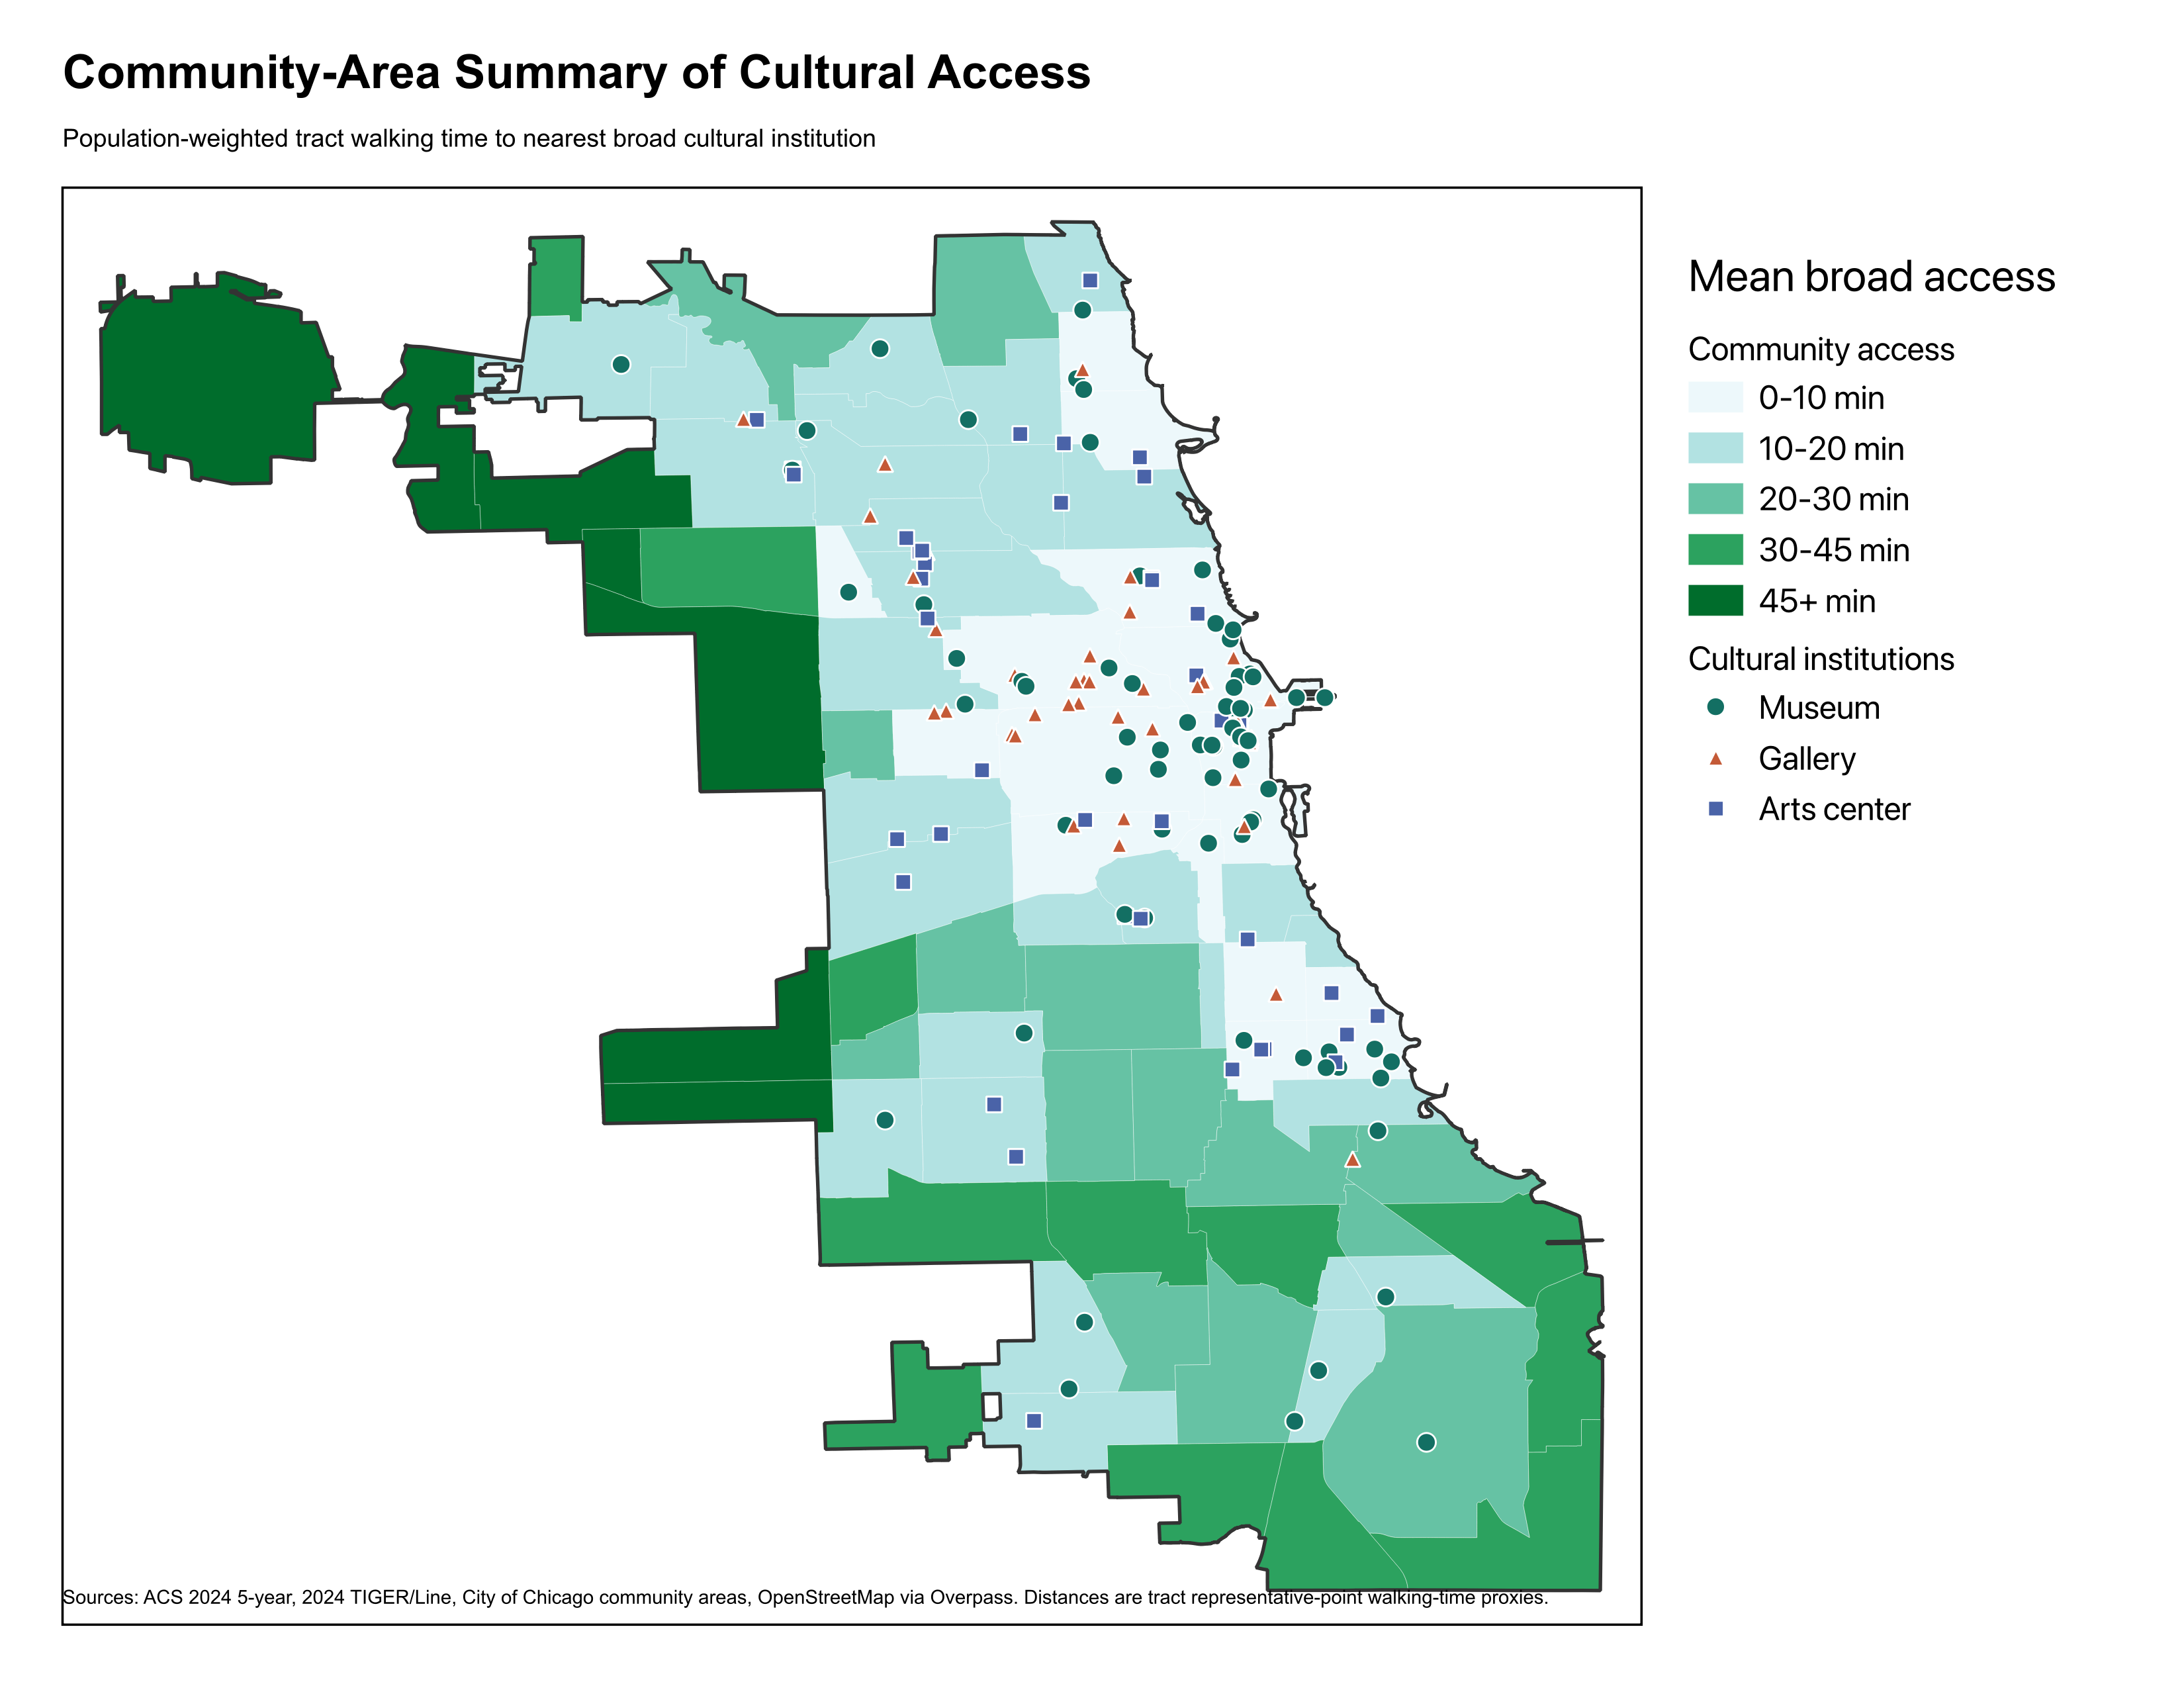
\includegraphics[width=\textwidth]{fig_04_community_access_qgis.png}
    \caption{Population-weighted community-area access to the nearest broad cultural institution.}
    \label{fig:community}
\end{figure}

The regression results support a more careful version of the hypothesis. The model explains about 34 percent of tract variation in broad walking-time access. Distance from the Loop is the strongest predictor: each additional mile from the Loop is associated with about 2.1 additional walking minutes to the nearest broad cultural institution, holding other variables constant. Population density is associated with shorter access. Black population share and Hispanic population share remain positively associated with longer access times: a full-range increase from 0 to 1 in Black share is associated with 7.4 additional minutes, and a full-range increase in Hispanic share is associated with 8.6 additional minutes. Poverty and no-vehicle rates are not positive predictors after controlling for centrality, density, race/ethnicity, and income.

\begin{figure}[H]
    \centering
    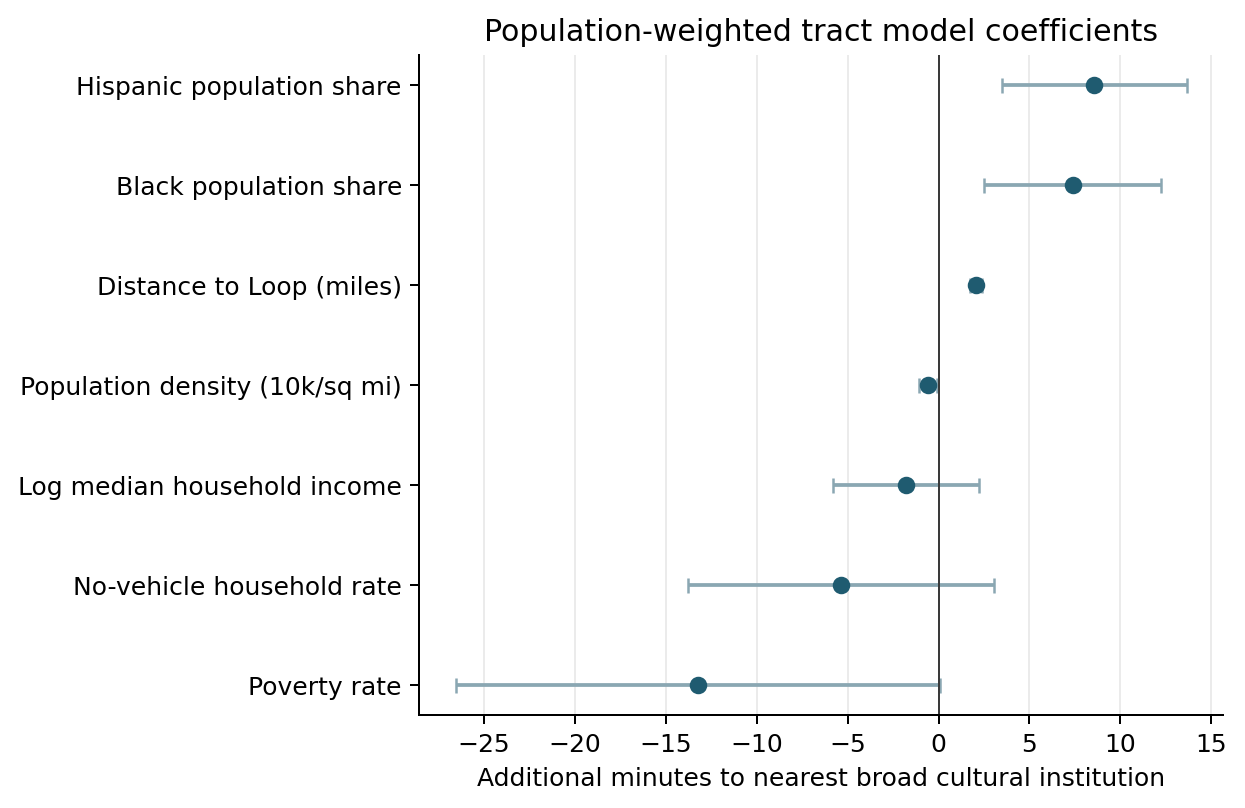
\includegraphics[width=0.92\textwidth]{fig_06_regression_coefficients.png}
    \caption{Population-weighted tract model coefficients with robust 95 percent confidence intervals.}
    \label{fig:coefficients}
\end{figure}

\section{Discussion and Limitations}

The evidence partially confirms the initial hypothesis. Museums and cultural institutions are not evenly distributed. The broad inventory shows meaningful access gaps, and the museum-only sensitivity analysis makes those gaps sharper. The clearest inequities are not captured by one variable such as poverty or car ownership. Instead, they appear through a combination of institutional clustering, distance from the Loop, lower density at the city's edges, and the racial and ethnic geography of Chicago.

Several limitations should qualify the findings. First, OpenStreetMap is an open, community-generated dataset. It is strong enough for a reproducible course project, but it may undercount smaller neighborhood heritage organizations or inconsistently classify galleries and arts centers. Second, the distance measure is a representative-point proximity proxy, not a street-network or scheduled-transit travel time. Third, the analysis does not include admission cost, hours, disability access, programming relevance, safety, language access, or whether residents feel welcomed by institutions. Fourth, ACS margins of error are preserved in the source workflow but not modeled in the final regression. These limitations are not minor; they define the next stage of a stronger cultural equity audit.

\section{Conclusion}

Chicago has abundant cultural institutions, but abundance is not the same as equitable spatial access. The citywide pattern is clustered, central, and uneven. Broad cultural access is relatively strong in the Loop, Near North Side, Near West Side, Hyde Park, and several adjacent areas, while many outer and historically marginalized communities have longer proximity times. Majority Black and majority Hispanic tracts have notably worse average access than majority White tracts, and that difference remains visible even after accounting for distance from the Loop and population density.

The policy implication is that cultural equity should be measured as neighborhood infrastructure, not only as audience outreach or citywide institutional prestige. If Chicago wants more equitable cultural access, the map points toward two complementary strategies: support existing neighborhood-based cultural organizations in lower-access areas, and improve multimodal access from outer South, West, Northwest, and Southwest Side communities to major cultural clusters. Future work should replace the straight-line proxy with GTFS-based transit times, validate the institution list with local cultural directories, and incorporate cost, hours, and programming to distinguish nominal proximity from meaningful access.

\begin{thebibliography}{9}

\bibitem[Brook(2016)]{brook2016}
Brook, O. (2016).
\newblock Spatial equity and cultural participation: How access influences attendance at museums and galleries in London.
\newblock \textit{Cultural Trends}, 25(1), 21--34. \url{https://doi.org/10.1080/09548963.2015.1134098}

\bibitem[Chen et~al.(2025)]{chen2025}
Chen, S.-Q., Zhang, J., Luan, W.-L., and Luo, X. (2025).
\newblock A GIS-based study on spatial pattern, accessibility and equity of urban cultural resources: A case study of red culture resources in Shanghai.
\newblock \textit{Buildings}, 15(13), 2268. \url{https://doi.org/10.3390/buildings15132268}

\bibitem[Geurs and van Wee(2004)]{geurs2004}
Geurs, K. T., and van Wee, B. (2004).
\newblock Accessibility evaluation of land-use and transport strategies: Review and research directions.
\newblock \textit{Journal of Transport Geography}, 12(2), 127--140. \url{https://doi.org/10.1016/j.jtrangeo.2003.10.005}

\bibitem[Hansen(1959)]{hansen1959}
Hansen, W. G. (1959).
\newblock How accessibility shapes land use.
\newblock \textit{Journal of the American Institute of Planners}, 25(2), 73--76. \url{https://doi.org/10.1080/01944365908978307}

\bibitem[Moldavanova et~al.(2021)]{moldavanova2021}
Moldavanova, A. V., Meloche, L., and Thompson, T. L. (2021).
\newblock Understanding the geography of access to cultural amenities: The case of Metropolitan Detroit.
\newblock \textit{Journal of Urban Affairs}. \url{https://doi.org/10.1080/07352166.2021.1886856}

\bibitem[Zhao et~al.(2023)]{zhao2023}
Zhao, X., Lee, J., and Hong, K. (2023).
\newblock A comparative analysis of museum accessibility in high-density Asian cities: Case studies from Seoul and Tokyo.
\newblock \textit{Buildings}, 13(8), 1886. \url{https://doi.org/10.3390/buildings13081886}

\bibitem[U.S. Census Bureau(2024a)]{censusacs2024}
U.S. Census Bureau. (2024a).
\newblock American Community Survey 2024 five-year detailed tables.
\newblock \url{https://api.census.gov/data/2024/acs/acs5}

\bibitem[U.S. Census Bureau(2024b)]{tiger2024}
U.S. Census Bureau. (2024b).
\newblock 2024 TIGER/Line shapefiles: Census tracts.
\newblock \url{https://www.census.gov/geographies/mapping-files/time-series/geo/tiger-line-file.html}

\bibitem[City of Chicago(2025)]{chicago2025}
City of Chicago. (2025).
\newblock Boundaries - Community Areas.
\newblock \url{https://data.cityofchicago.org/Facilities-Geographic-Boundaries/Boundaries-Community-Areas/igwz-8jzy}

\bibitem[OpenStreetMap contributors(2026)]{osm2026}
OpenStreetMap contributors. (2026).
\newblock OpenStreetMap data extracted via Overpass API. Data available under the Open Database License.
\newblock \url{https://www.openstreetmap.org/copyright}

\end{thebibliography}

\end{document}
